\section{Comparison of CV models}
\label{sxn:cv}

In this section, we examine empirical quality metrics described in Section~\ref{sxn:methods} for several CV model architecture series.
This includes the VGG, ResNet, and DenseNet series of models, each of which consists of several pretrained DNN models, trained on the full ImageNet~\cite{imagenet} dataset, and each of which is distributed with the current opensource pyTorch framework (version 1.4)~\cite{pytorch}.
This also includes a larger set of ResNet models, trained on the ImageNet-1K dataset~\cite{imagenet}, provided on the OSMR ``Sandbox for training convolutional networks for computer vision''~\cite{osmr}, which we call the ResNet-1K series.

We perform \emph{coarse model analysis}, comparing and contrasting the four model series, and predicting trends in model quality. 
We also perform \emph{fine layer analysis}, as a function of depth for these models, illustrating that PL-based metrics can provide novel insights among the VGG, ResNet/ResNet-1K, and DenseNet architectures. 


\paragraph{Average Quality Metrics versus Reported Test Accuracies.}

We have examined the performance of the four quality metrics (Log Frobenius norm, Log Spectral norm, Weighted Alpha, and Log $\alpha$-Norm) applied to each of the VGG, ResNet, ResNet-1K, and DenseNet series.
To start, Figure~\ref{fig:vgg-metrics} considers the VGG series (in particular, the pretrained models VGG11, VGG13, VGG16, and VGG19, with and without BN), and it plots the four quality metrics versus the reported test accuracies~\cite{pytorch},% 
\footnote{That is, these test accuracies have been previously reported and made publicly-avaiable by others.  We take them as given, and we do not attempt to reproduce/verify them, since we do not permit ourselves any access to training/test data.}
as well as a basic linear regression line. 
%with the Root Mean Squared Error (RMSE) shown, \michael{XXX.  WHERE IS RMSE.  IN THAT TABLE?}
All four metrics correlate quite well with the reported Top1 accuracies, with smaller norms and smaller values of $\hat{\alpha}$ implying better generalziation (i.e., greater accuracy, lower error). 
While all four metrics perform well, notice that the Log $\alpha$-Norm metric ($\log\Vert\mathbf{W}\Vert_{\alpha}^{\alpha}$) performs best (with an RMSE of $0.42$, see Table~\ref{table:cv-models}); and the Weighted Alpha metric ($\hat\alpha =\alpha\log\lambda_{max} $), which is an approximation to the Log $\alpha$-Norm metric~\cite{MM20_unpub_work}, performs second best (with an RMSE of $0.48$, see Table~\ref{table:cv-models}).

\begin{figure}[t]
    \centering
    \subfigure[Log Frobenius Norm, VGG ]{
        %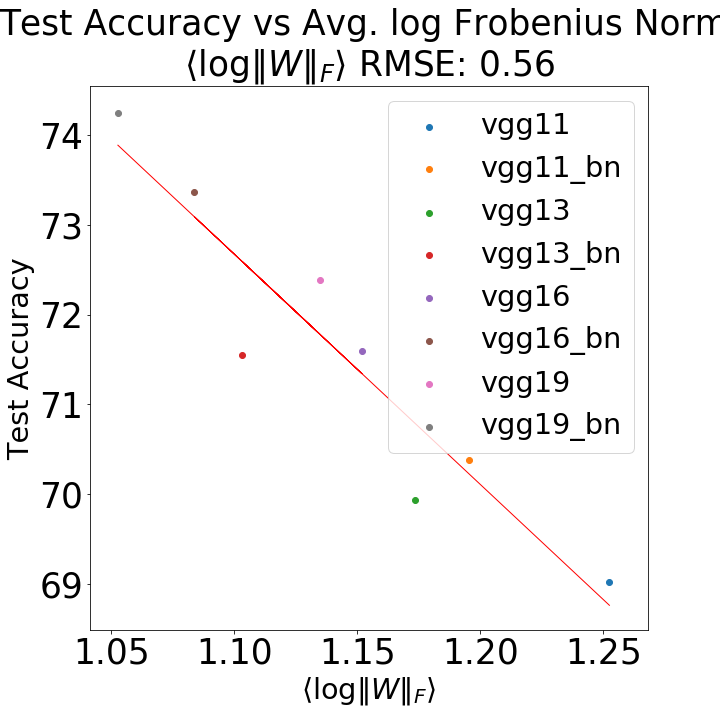
\includegraphics[width=5cm]{img/VGG_lognorm_accs.png}
        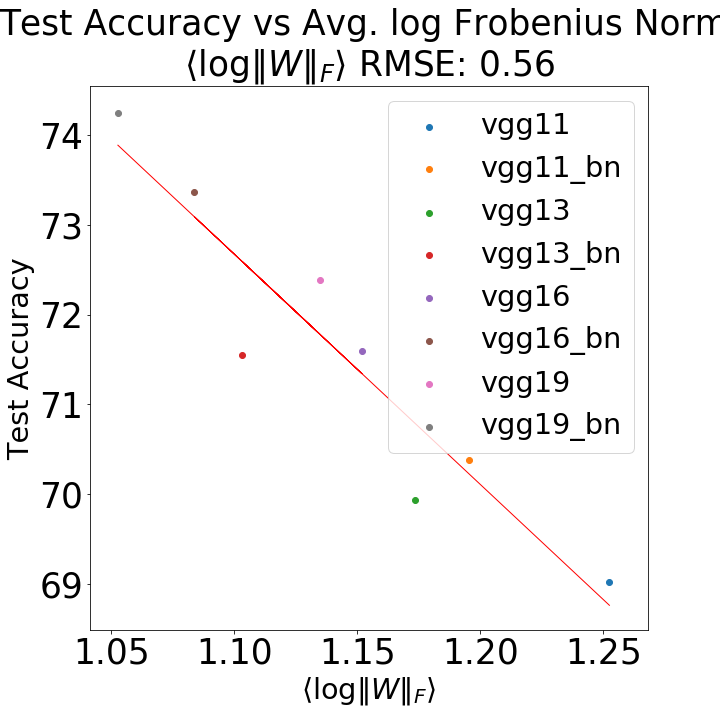
\includegraphics[width=4.0cm]{img/VGG_lognorm_accs.png}
        \label{fig:vgg-fnorm}
    }
    %\qquad
    \subfigure[Log Spectral Norm, VGG ]{
        %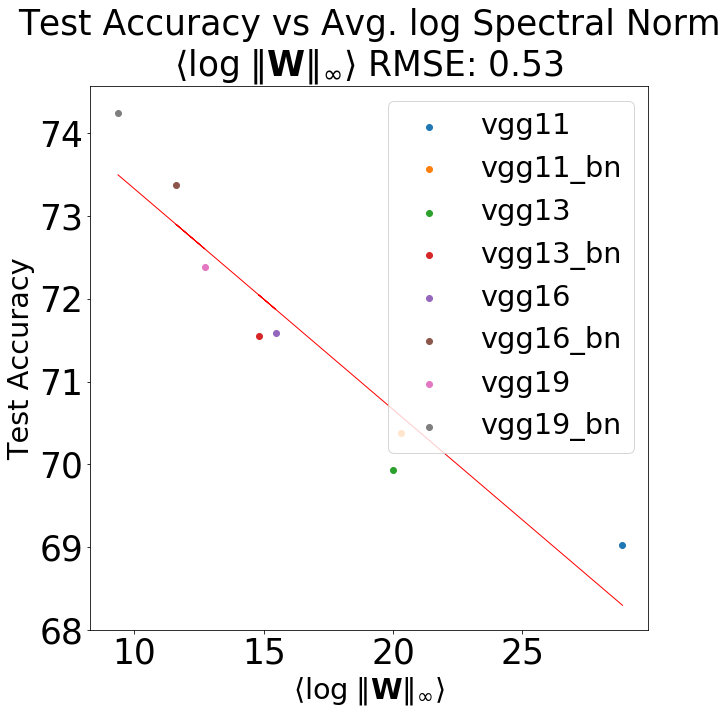
\includegraphics[width=4.9cm]{img/VGG_spectralnorm_accs.png}
        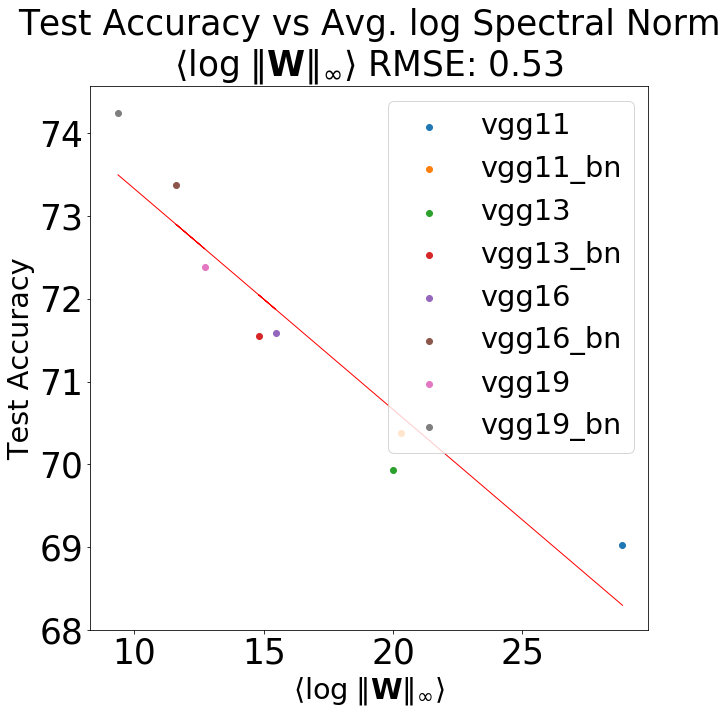
\includegraphics[width=4.0cm]{img/VGG_spectralnorm_accs.png}
        \label{fig:vgg-snorm}
    }
    %\qquad
    \subfigure[ Weighted Alpha, VGG ]{
        %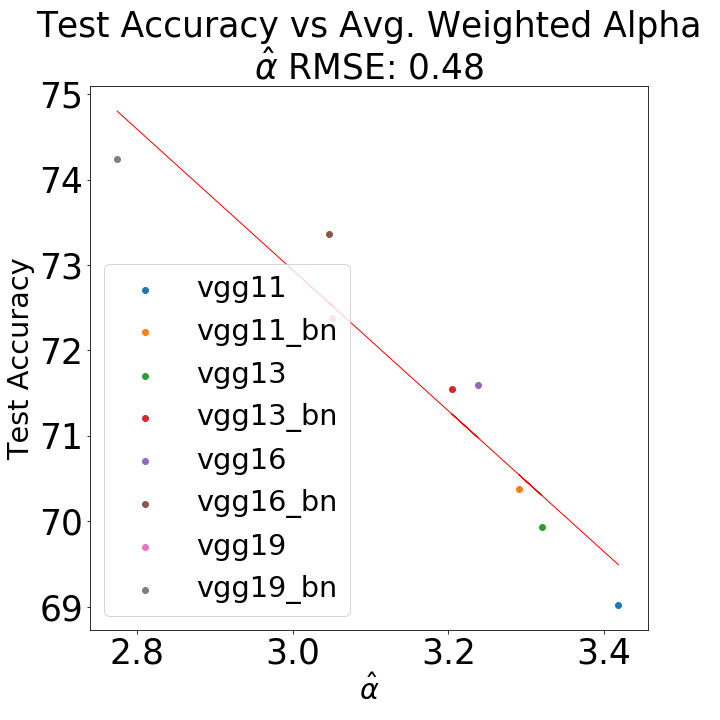
\includegraphics[width=4.9cm]{img/VGG_alpha_weighted_accs.png}
        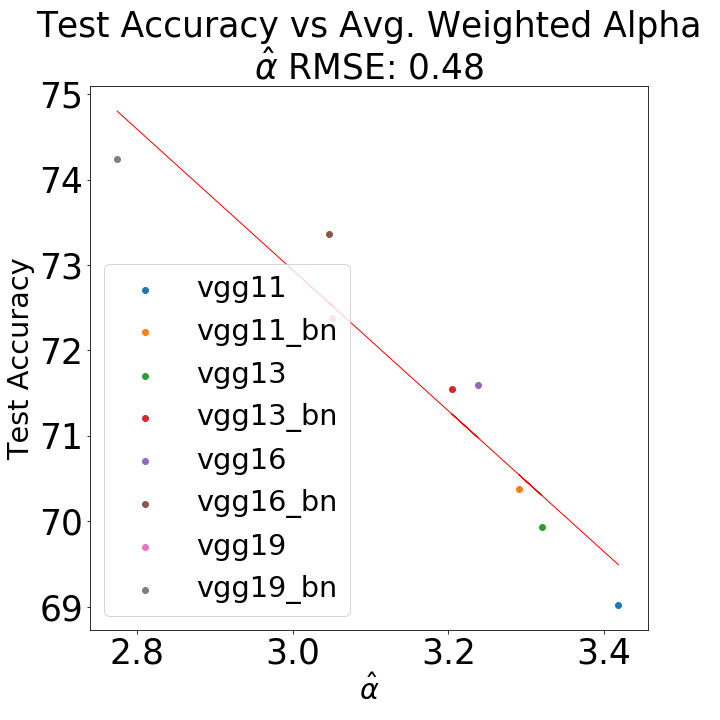
\includegraphics[width=4.0cm]{img/VGG_alpha_weighted_accs.png}
        \label{fig:vgg-walpha}
    }
    %\qquad
    \subfigure[Log $\alpha$-Norm, VGG ]{
        %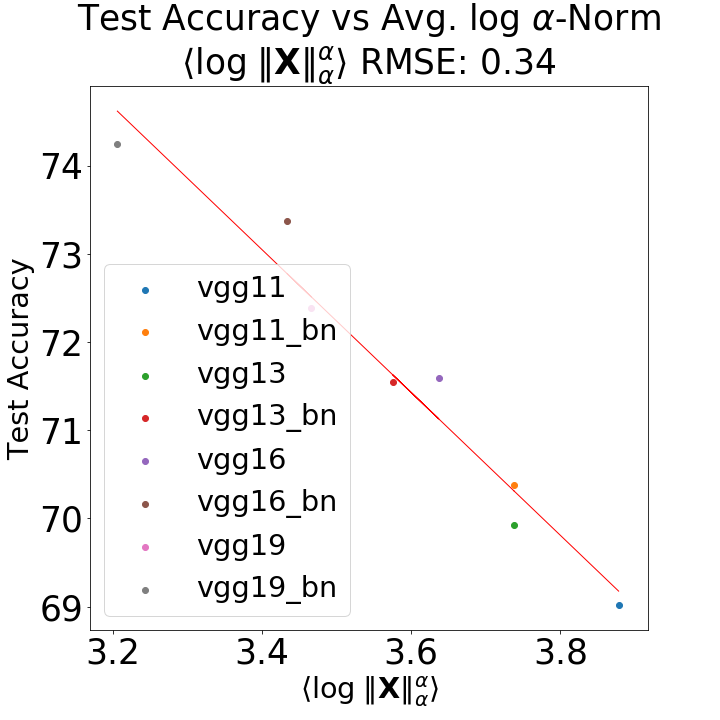
\includegraphics[width=4.9cm]{img/VGG_logpnorm_accs.png}
        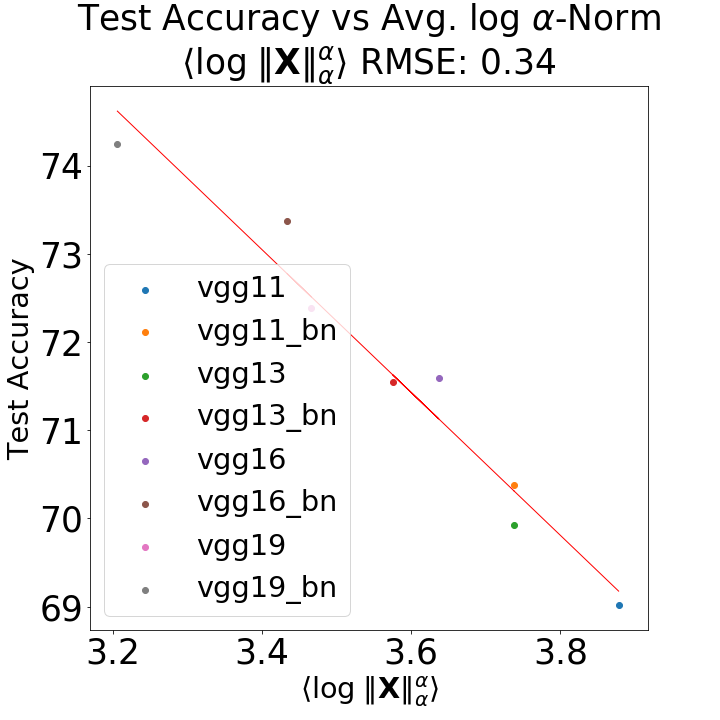
\includegraphics[width=4.0cm]{img/VGG_logpnorm_accs.png}
        \label{fig:vgg-pnorm}
    }
    \caption{Comparison of Average Log Norm and Weighted Alpha quality metrics versus reported test accuracy for pretrained VGG models (with and without BN), trained on ImageNet, available in pyTorch (v1.x).  Metrics fit by linear regression, RMSE reported. }
    \label{fig:vgg-metrics}
\end{figure}


\begin{figure}[t]
    \centering

    \subfigure[ ResNet, Log $\alpha$-Norm ]{
        %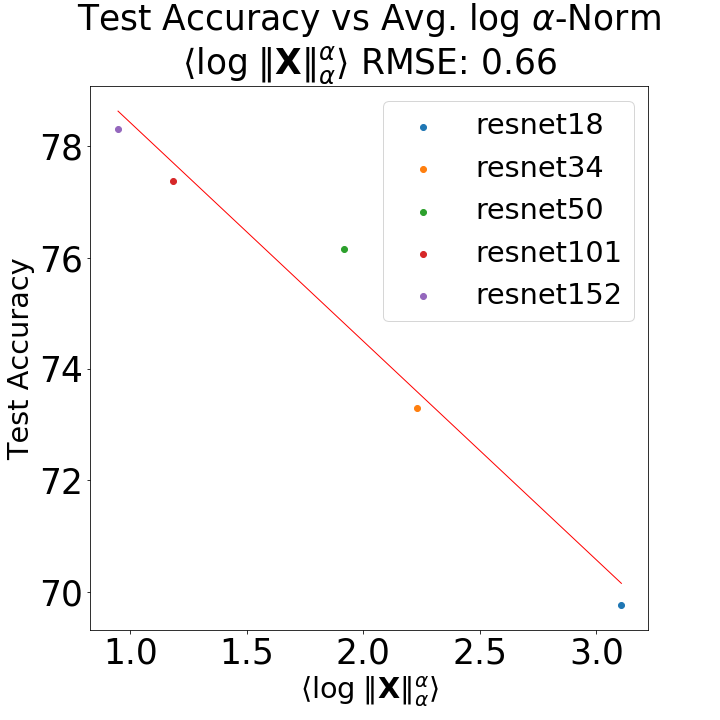
\includegraphics[width=4.2cm]{img/ResNet_logpnorm_accs.png}
        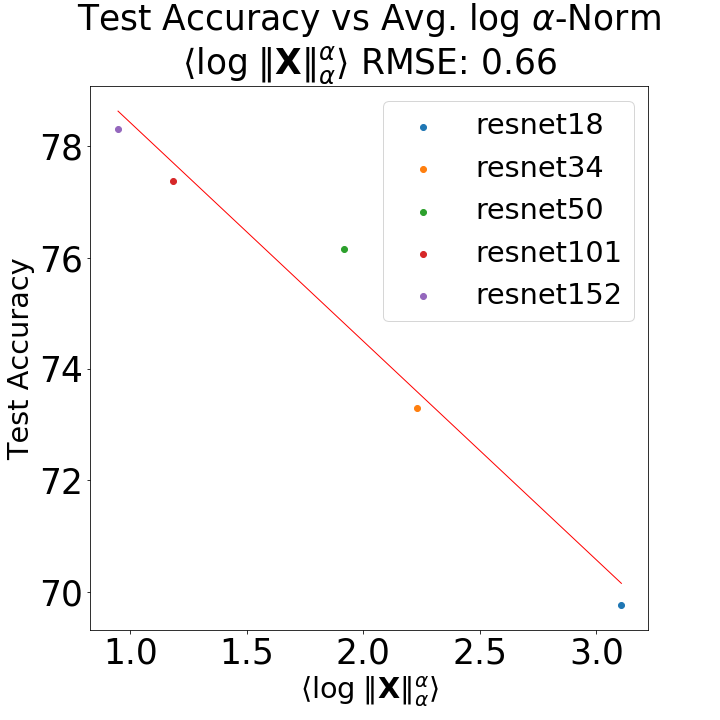
\includegraphics[width=4.0cm]{img/ResNet_logpnorm_accs.png}
        \label{fig:resnet-accuracy}
    }
    %\qquad
    \subfigure[ ResNet-1K, Log $\alpha$-Norm ]{
        %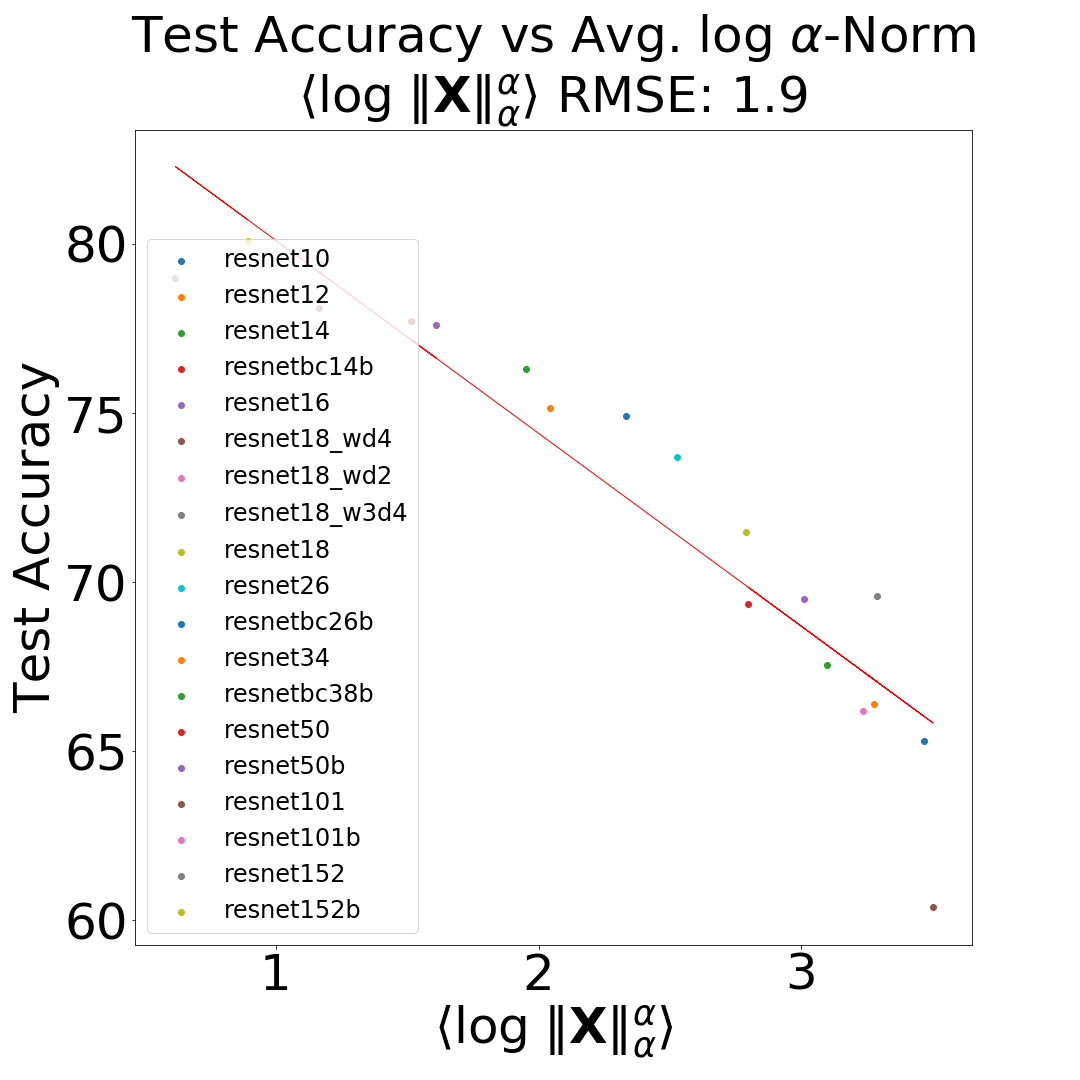
\includegraphics[width=4.5cm]{img/ResNet-1K_logpnorm_accs.png}
        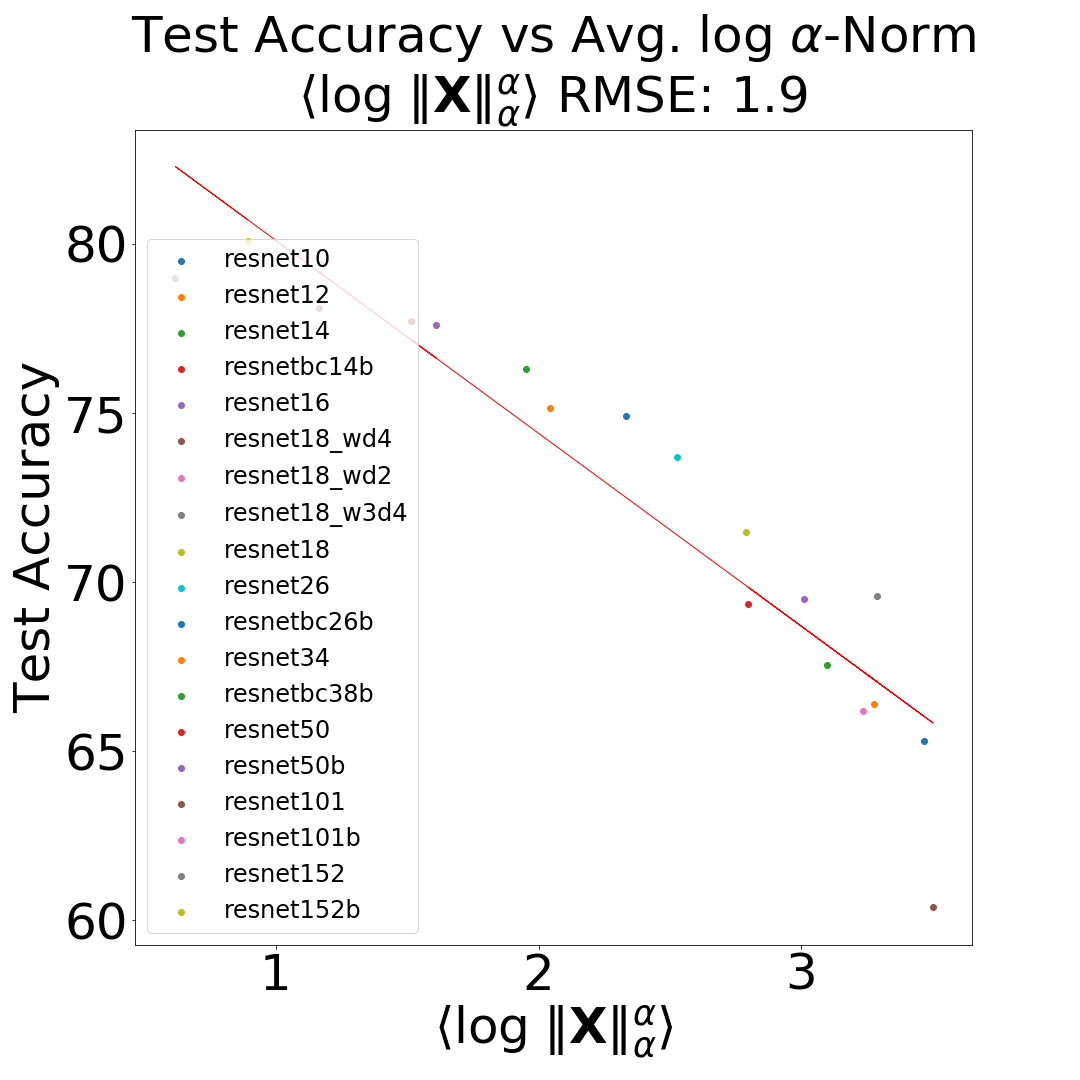
\includegraphics[width=4.0cm]{img/ResNet-1K_logpnorm_accs.png}
        \label{fig:resnet1k-accuracy}
    }
    %\qquad
    %\subfigure[ DenseNet, Log $\alpha$-Norm ]{
    %    %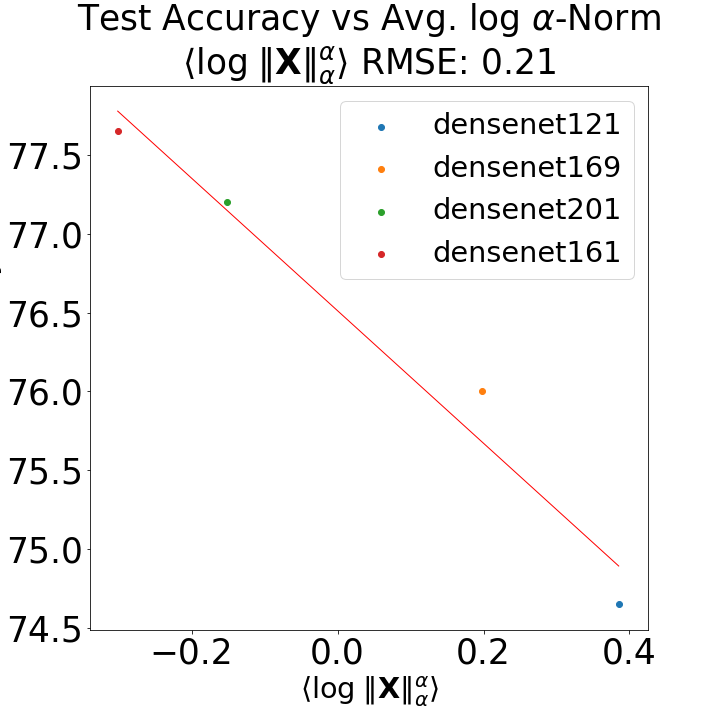
\includegraphics[width=4.4cm]{img/DenseNet_logpnorm_accs.png}
    %    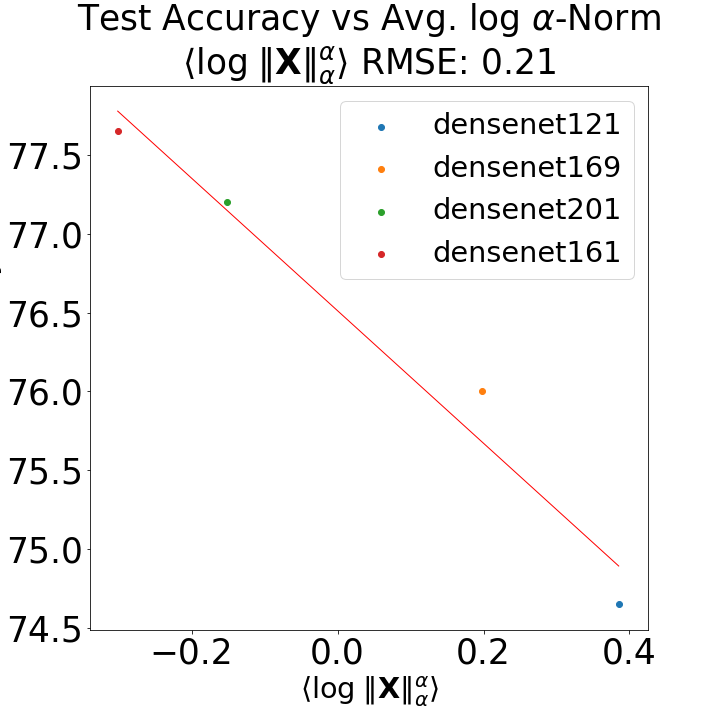
\includegraphics[width=4.0cm]{img/DenseNet_logpnorm_accs.png}
    %    \label{fig:densenet-accuracy}
    %}
    \caption{Comparison of Avergage $\alpha$-Norm quality metric ($\langle\log\Vert\mathbf{X}\Vert_{\alpha}^{\alpha}\rangle$) versus reported Top1 test accuracy for the ResNet and ResNet-1K pretrained (pyTorch) models. }
%, and DenseNet models. }The corresponding results for VGG are shown in Figure~\ref{fig:vgg-pnorm}.  }
    \label{fig:cv2-accuracy}
\end{figure}


%MM% \begin{figure}
%MM% \centering
%MM% \begin{minipage}[b]{.22\textwidth}
%MM% %<Code for the first figure>
%MM% XXX
%MM% \caption{Caption}\label{label-a}
%MM% \end{minipage}\qquad
%MM% \begin{minipage}[b]{.22\textwidth}
%MM% %<Code for the second figure>
%MM% XXX
%MM% \caption{Caption}\label{label-b}
%MM% \end{minipage}
%MM% \end{figure}


\begin{table}[t]
\small
\begin{center}
%\begin{tabular}{|p{1in}|c|c|c|c|c|}
\begin{tabular}{|p{0.65in}|c|c|c|c|c|}
%\begin{tabular}{|l|c|c|c|c|c|}
\hline
 Series    &\#   & $\langle\log\Vert\mathbf{W}\Vert_{F}\rangle$ & $\langle\log\Vert\mathbf{W}\Vert_{\infty}\rangle$ & $\hat{\alpha}$ & $\langle\log\Vert\mathbf{X}\Vert^{\alpha}_{\alpha}\rangle$ \\
\hline
 VGG       &  6 & 0.56 & 0.53 & 0.48          & \textbf{0.42}  \\
 ResNet    &  5 & 0.9  & 1.4  & \textbf{0.61} & 0.66           \\
 ResNet-1K & 19 & 2.4  & 3.6  & \textbf{1.8}  & 1.9            \\
 DenseNet  &  4 & 0.3  & 0.26 & \textbf{0.16} & 0.21           \\
\hline
\end{tabular}
\end{center}
\caption{RMSE (smaller is better) for linear fits of 
         %Average Log Norm and Weighted Alpha 
         quality metrics to reported Top1 test error for pretrained models in each architecture series.  Column \# refers to number of models.  VGG, ResNet, and DenseNet were pretrained on ImageNet, and ResNet-1K was pretrained on ImageNet-1K. 
}
\label{table:cv-models}
\end{table}

See Table~\ref{table:cv-models} for a summary of results for Top1 accuracies for all four metrics on for the VGG, ResNet, and DenseNet series.
Similar results (not shown) are obtained for the Top5 accuracies.
Overall, for the the ResNet, ResNet-1K, and DenseNet series, all metrics perform relatively well, the Log $\alpha$-Norm metric performs second best, and the Weighted Alpha metric performs best.
These model series are all well-trodden, and our results indicate that norm-based metrics and PL-based metrics can both distinguish among ``good-better-best'' models, with PL-based metrics performing somewhat (i.e., quantitatively) better.

The DenseNet series has similar behavior to what we see in Figures~\ref{fig:vgg-metrics} and~\ref{fig:cv2-accuracy} for the other models.
However, as noted in Table~\ref{table:cv-models}, it has only 4 data points.  
In our larger analysis, in Section~\ref{sxn:all_cv_models}, we will only include series with 5 or more models.
%For completemnss and reproducibility here, the DenseNet Log $\alpha$-Norm plot is given in Appendix~\ref{sxn:appendix}.
(Note that these and many other such plots can be seen on our publicly-available~repo.)


\paragraph{Variation in Data Set Size.}

We are interested in how our four quality metrics depend on data set size.
To examine this, we look at results on ResNet versus ResNet-1K.
See Figure~\ref{fig:cv2-accuracy}, which plots and compares the Log $\alpha$-Norm metric 
%% MM: From Table 1 it is slightly worse than alpha-hat and we say that below %% --the best performing metric--
for the full ResNet model, trained on the full ImageNet dataset, against the ResNet-1K model, which has been trained on a much smaller ImageNet-1K data set.
The Log $\alpha$-Norm is much better than the Log Frobenius/Spectral norm metrics (although, as Table~\ref{table:cv-models} shows, it is actually slightly worse than the Weighted Alpha metric).
The ResNet series has strong correlation, with an RMSE of $0.66$, whereas the ResNet-1K series also shows good correlation, but has a much larger RMSE of $1.9$.
(Other metrics exhibit similar behavior.)
As expected, the higher quality data set shows a better fit, even with fewer data points.


\paragraph{Layer Analysis: Metrics as a Function of Depth.}

We can learn much more about a pretrained model by going beyond average values of quality metrics to examining quality metrics for each layer weight matrix, $\mathbf{W}$, as a function of depth (or layer id).  % in the network. 
%The most interesting results are seen when we 
For example, we can 
plot (just) the PL exponent, $\alpha$, for each layer, %
%\footnote{That is, here we consider just $\alpha$ for each layer, i.e., not $\hat{\alpha}$ or $\Vert\mathbf{W}\Vert^{\alpha}_{\alpha}$.} 
as a function of depth.
%
See Figure~\ref{fig:3models-alpha-layers}, which plots $\alpha$ for each layer (the first layer corresponds to data, the last layer to labels) for the least accurate (shallowest) and most accurate (deepest) model in each of the VGG (no BN), ResNet, and DenseNet series.
(Again, much more detailed set of plots is available at our repo; but note that the corresponding layer-wise plots for Frobenius and Spectral norms are much less interesting than the results we present here.)

\begin{figure}[t]
    \centering

    \subfigure[ VGG ]{
        %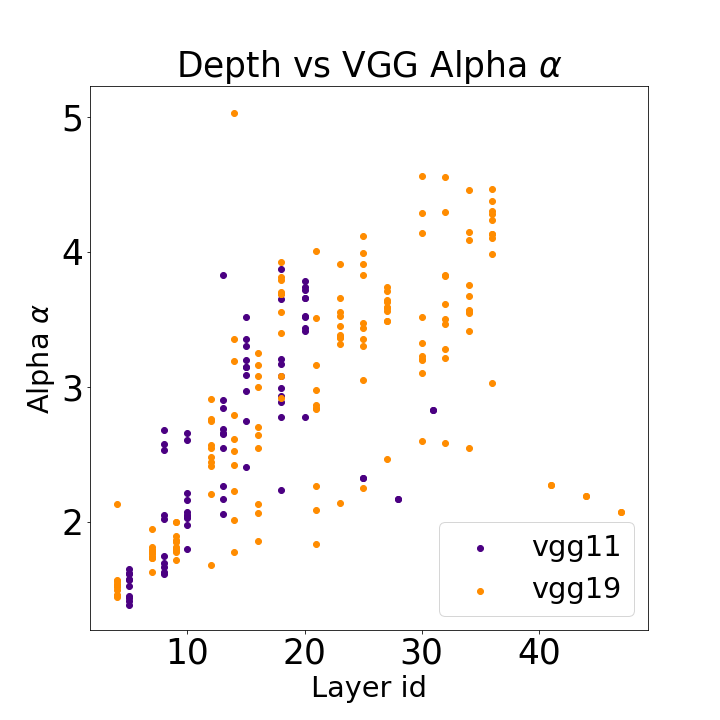
\includegraphics[width=4.5cm]{img/VGG_fnl_alpha_depth.png} 
        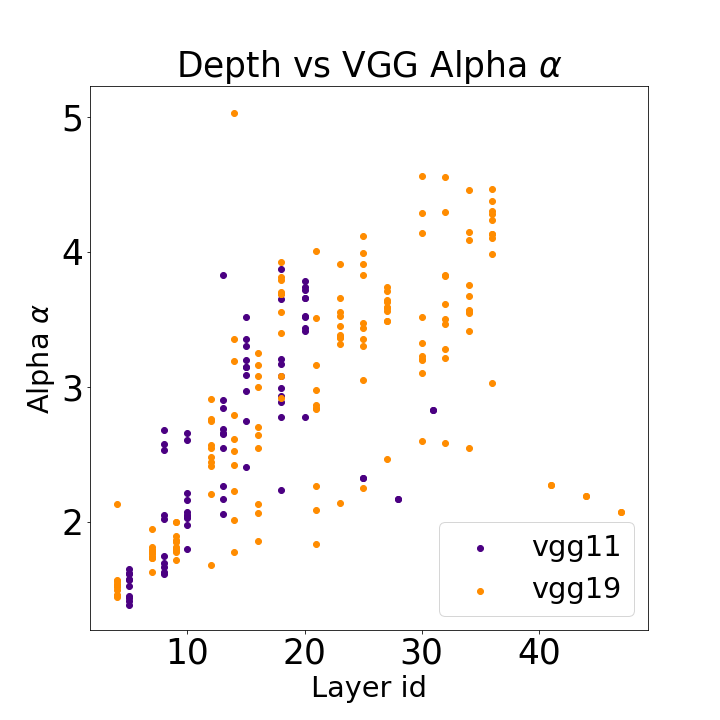
\includegraphics[width=4.0cm]{img/VGG_fnl_alpha_depth.png} 
                \label{fig:vgg-alpha-layers}
    }
    %\qquad
    \subfigure[ ResNet-1K ]{
        %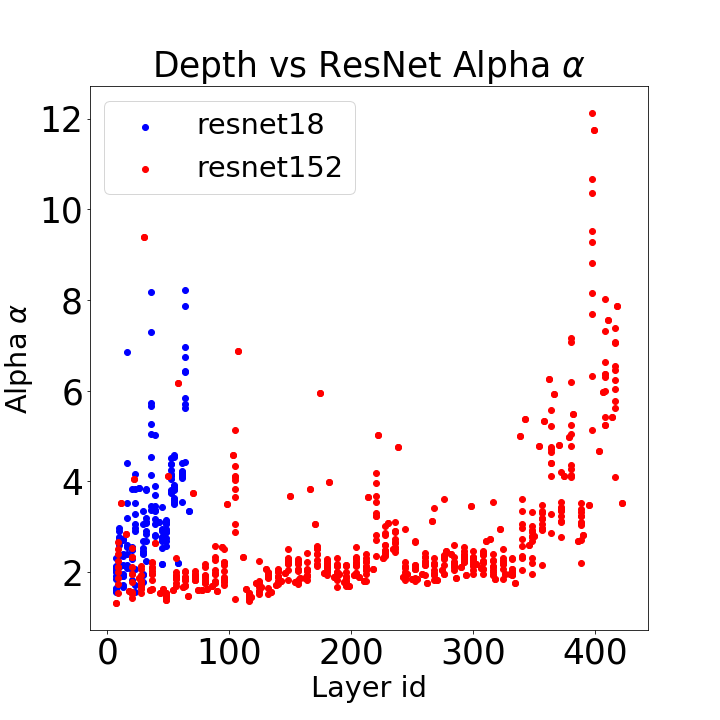
\includegraphics[width=4.5cm]{img/ResNet_fnl_alpha_depth.png} 
        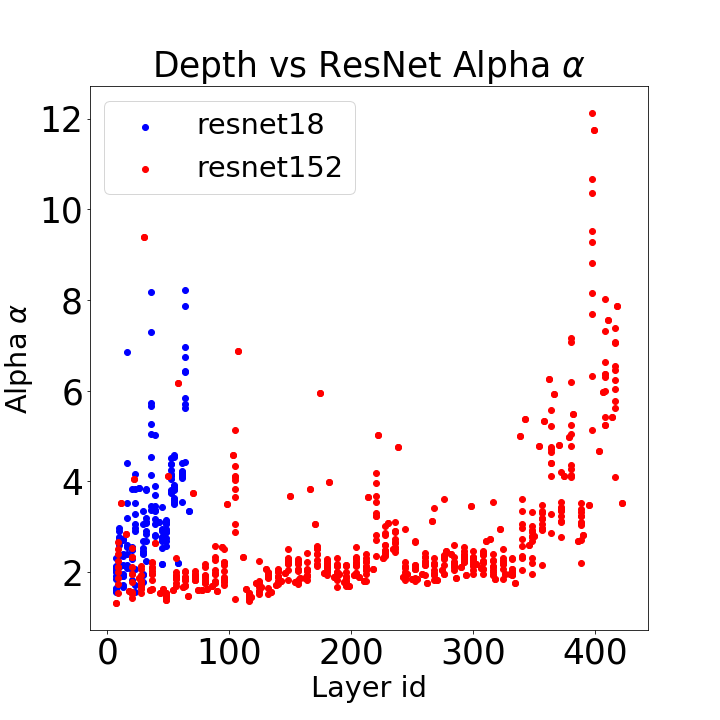
\includegraphics[width=4.0cm]{img/ResNet_fnl_alpha_depth.png} 
        \label{fig:resnet-alpha-layer}
    }
    %\qquad
    \subfigure[ DenseNet ]{
        %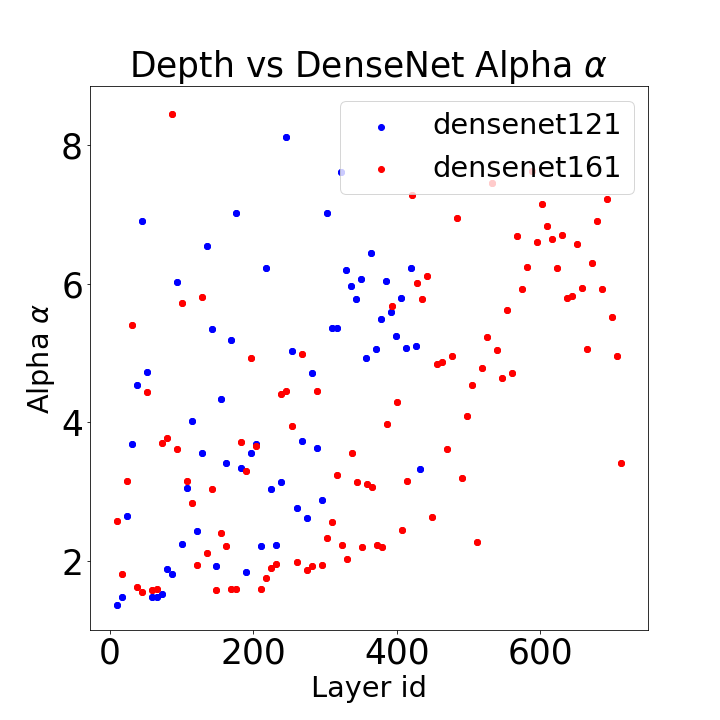
\includegraphics[width=4.5cm]{img/DenseNet_fnl_alpha_depth.png} 
        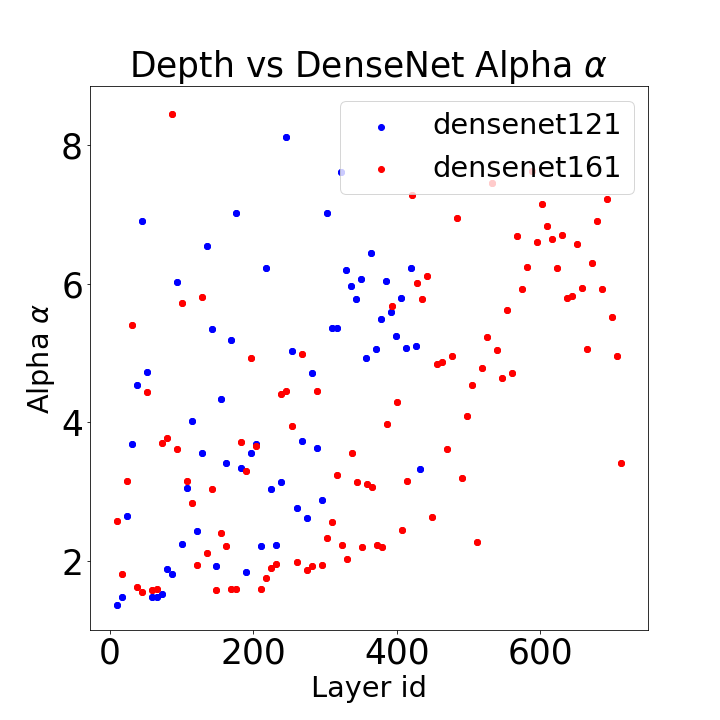
\includegraphics[width=4.0cm]{img/DenseNet_fnl_alpha_depth.png} 
        \label{fig:densenet-alpha-layer}
    
}    \subfigure[ ResNet-1K (overlaid) ]{
        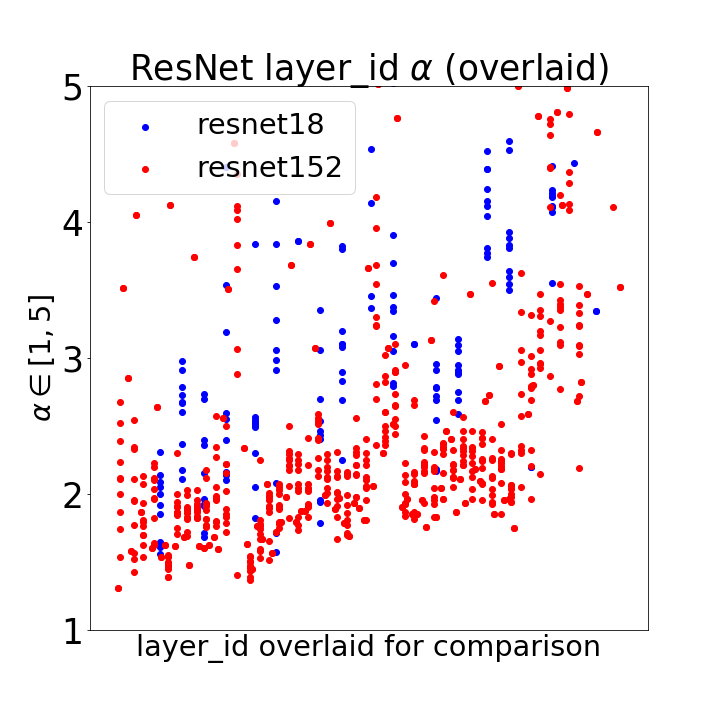
\includegraphics[width=4.0cm]{img/resnet_alpha_overlaid_depth.png} 
        \label{fig:resnet_alpha_overlaid_depth}
    }
    \caption{PL exponent ($\alpha$) versus layer id, for the least and the most accurate models in VGG (a), ResNet (b), and DenseNet (c) series. 
             (VGG is without BN; and note that the Y axes on each plot are different.)  
             Subfigure (d) displays the ResNet models (b), zoomed in to $\alpha\in[1,5]$, and with the layer ids overlaid on the X-axis, from smallest to largest, to
             allow a more detailed analysis for the most strongly correlated layers.
             Notice that ResNet152 exhibits different and much more stable behavior of $\alpha$ across layers.
             This contrasts with how both VGG models gradually worsen in deeper layers and how the DenseNet models are much more erratic.  
             In the text, this is interpreted in terms of \emph{Correlation Flow}.
            }
    \label{fig:3models-alpha-layers}
\end{figure}

In the VGG models, Figure~\ref{fig:vgg-alpha-layers} shows that the PL exponent $\alpha$ systematically increases as we move down the network, from data to labels, in the Conv2D layers, starting with $\alpha\lesssim 2.0$ and reaching all the way to $\alpha\sim 5.0$; and then, in the last three, large, fully-connected (FC) layers, $\alpha$ stabilizes back down to $\alpha\in[2,2.5]$.
This is seen for all the VGG models (again, only the shallowest and deepest are shown in this figure), indicating that the main effect of increasing depth is to increase the range over which $\alpha$ increases, thus leading to larger $\alpha$ values in later Conv2D layers of the VGG models.
This is quite different than the behavior of either the ResNet-1K models or the DenseNet models.

For the ResNet-1K models, Figure~\ref{fig:resnet-alpha-layer} shows that $\alpha$ also increases in the last few layers (more dramatically, in fact, than for VGG, observe the differing scales on the Y axes).
However, as the ResNet-1K models get deeper, there is a wide range over which $\alpha$ values tend to remain quite small.
%\michael{Can we say something about exceptions which are larger than for VGG or DenseNet.}
%\charles{You have the same plots I do..what do you want to say >}
%\michael{Are they small or different types of layers or something?}
%\charles{Not that I am aware of.  Ill think on it}
This is seen for other models in the ResNet-1K series, but it is most pronounced for the larger ResNet-1K (152) model, where $\alpha$ remains relatively stable at $\alpha\sim 2.0$, from the earliest layers all the way until we reach close to the final layers.  

For the DenseNet models, Figure~\ref{fig:densenet-alpha-layer} shows that $\alpha$ tends to increase as the layer id increases, in particular for layers toward the end.
While this is similar to what is seen in the VGG models, with the DenseNet models, $\alpha$ values increase almost immediately after the first few layers, and the variance is much larger (in particular for the earlier and middle layers, where it can range all the way to $\alpha\sim 8.0$) and much less systematic throughout the network.

%Recall the differences---in particular, the number of residual connections---between the VGG, ResNet, and DenseNet architectures.
%VGG, while a fine model in many ways, was limited by needing massive FC layers at the end of the model, requiring significant memory and computational resources, and it's poor conditioning led to problems with vanishing gradients.  
%The empirical manifestations of this (on weight matrices) are that fitted $\alpha$ values get much worse for deeper layers.
%%\ncyan{
\paragraph{Comparison of VGG, ResNet, and DenseNet Architectures.}
We can interpret these observations by recalling the architectural differences between the VGG, ResNet, and DenseNet architectures,
and, in particular, the number of of residual connections. VGG resembles the  traditional convolutional architectures,
such as LeNet5, and consists of several [Conv2D-Maxpool-ReLu] blocks, followed by 3 large Fully Connected (FC) layers.
ResNet greatly improved on VGG by replacing the large FC layers, shrinking the Conv2D blocks, and introducing \emph{residual connections}.
This optimized approach allows for greater accurary with far fewer parameters (and GPU memory requirements), and
ResNet models of up to 1000 layers have been trained.\cite{resnet1000}.
%%}
We conjuecture that the effeciency and effectivness of ResNet is reflected in the smaller and more stable $\alpha\sim 2.0$, across nearly all layers, indicating that the inner layers are very well correlated and strongly optimized.
Contrast this with the DenseNet models, which contains many connections between every layer.
Our results (large $\alpha$, meaning they even a HT model is probably a poor fit) suggest that DenseNet has too many connections, diluting high quality interactions across layers, and leaving many layers very poorly optimized.


\paragraph{Correlation Flow.}

More generally, we can understand the results presented in Figure~\ref{fig:3models-alpha-layers} in terms of what we will call the \emph{Correlation Flow} of the model. 
Recall that the average Log $\alpha$-Norm metric and the Weighted Alpha metric are based on HT-SR Theory~\cite{MM18_TR, MM19_HTSR_ICML, MM20_SDM}, which is in turn based on ideas from the statisical mechanics of heavy tailed and strongly correlated systems~\cite{BouchaudPotters03, SornetteBook, BP11, bun2017}. 
There, one expects the weight matrices of well-trained DNNs will exhibit correlations over many size scales. 
Their ESDs can be well-fit by a (truncated) PL, with exponents $\alpha\in[2,4]$.
Much larger values $(\alpha\gg 5\;\mbox{or}\;6)$ may reflect poorer PL fits, whereas smaller values $(\alpha\sim 2)$, are associated with models that generalize better.
%, but the presence of many adjacent layers with relatively good PL fits \emph{suggests} that those adjacent layers ``impedance match'' well and that the correlations that are captured by one layer propagate well to subsequent layers.
Informally, one would expect a DNN model to perform well when it fascilitates the propagation of information/features across layers.
Previous work argues this by computing the gradients over the input data.
In the absence of training/test data, one might hope that this leaves empirical signatures on weight matrices, and thus we can to try to quantify this by measuring the PL properties of weight matrices.
In this case, smaller $\alpha$ values correspond to layers in which correlations across multiple scales are better captured~\cite{MM18_TR,SornetteBook}, and we expect that small $\alpha$ values that are stable across multiple layers enable better \emph{correlation flow} through the network.
We have seen this in many models, including those shown in Figure~\ref{fig:3models-alpha-layers}.


\begin{figure}[t]
   \centering
   \subfigure[$\lambda_{max}$ for ResNet20 layers]{
      %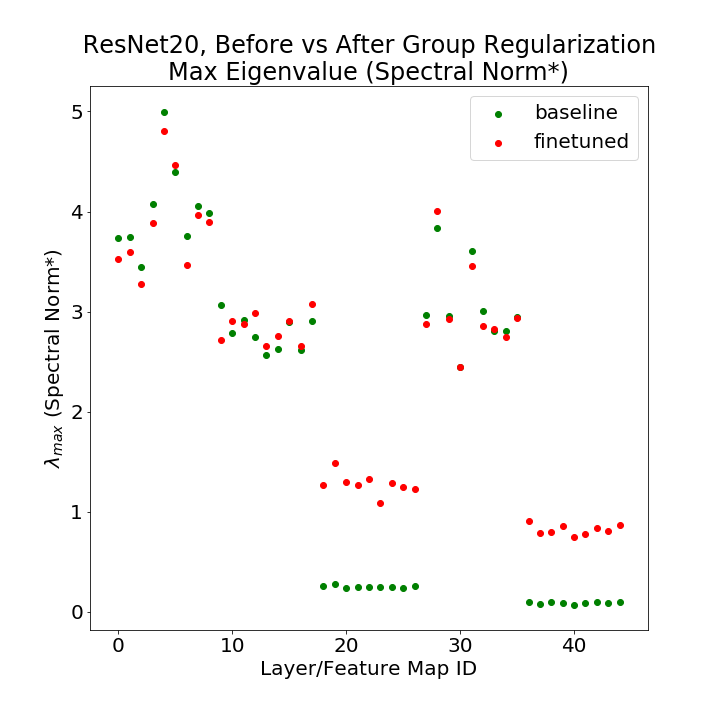
\includegraphics[scale=0.14]{img/resnet4d_maxev.png}
      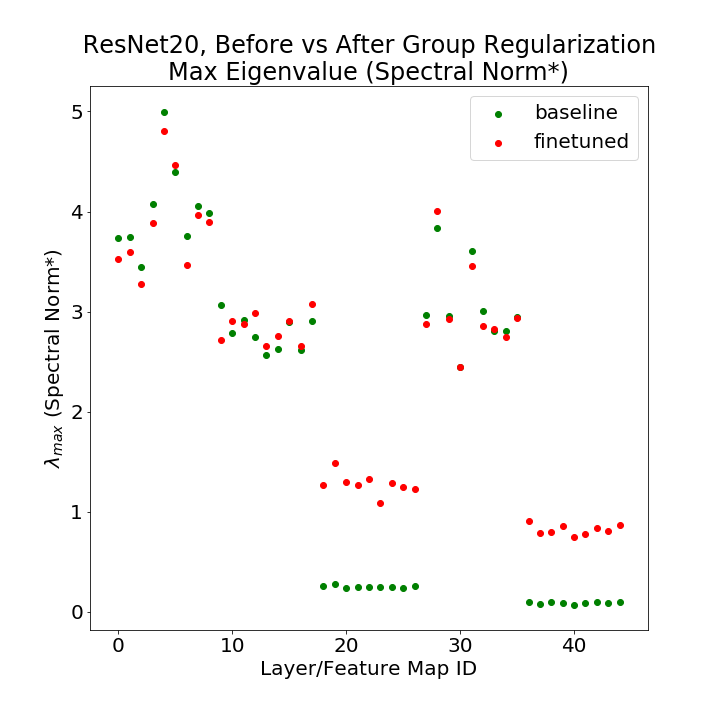
\includegraphics[width=4.0cm]{img/resnet4d_maxev.png}
      %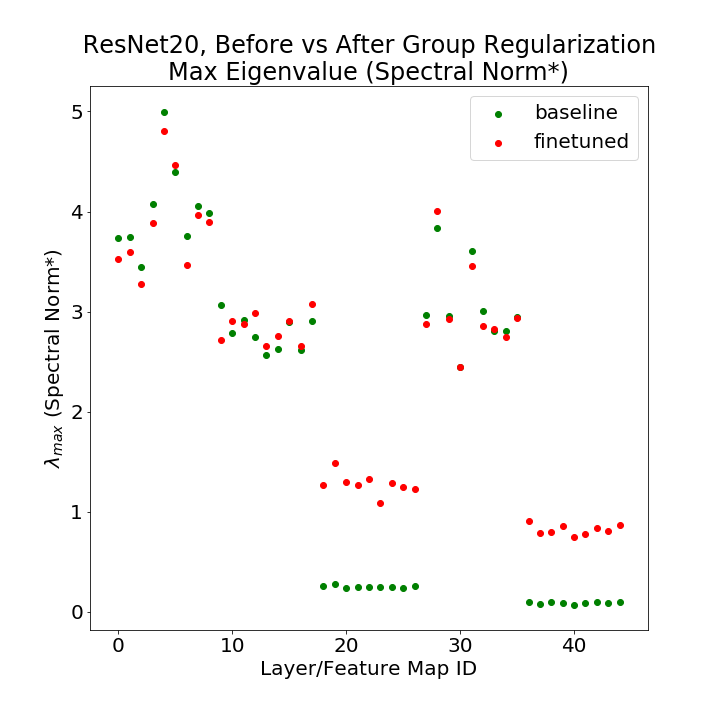
\includegraphics[width=4.5cm]{img/resnet4d_maxev.png}
      \label{fig:resnet204Dmaxev}
   }
   %\qquad
   \subfigure[$\alpha$ for ResNet20 layers]{
      %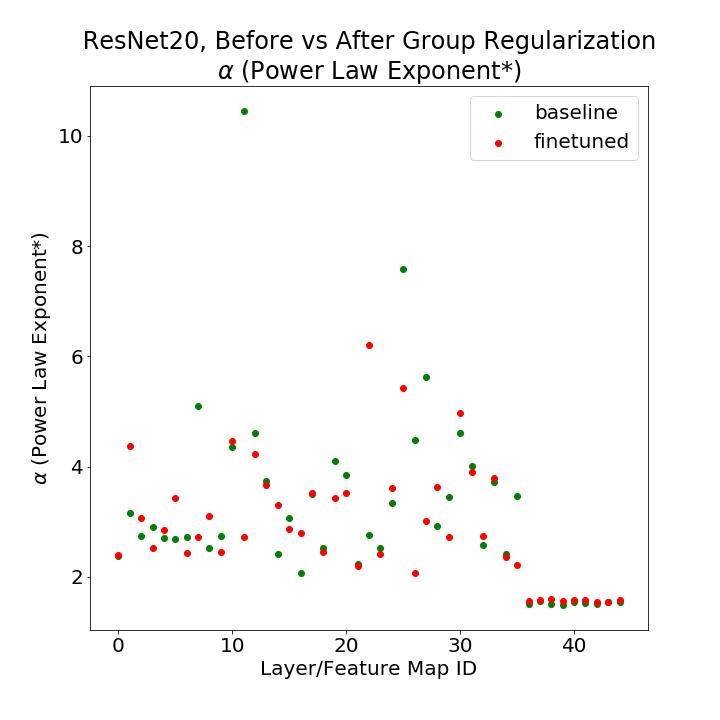
\includegraphics[scale=0.14]{img/resnet4d_alphas.png}
      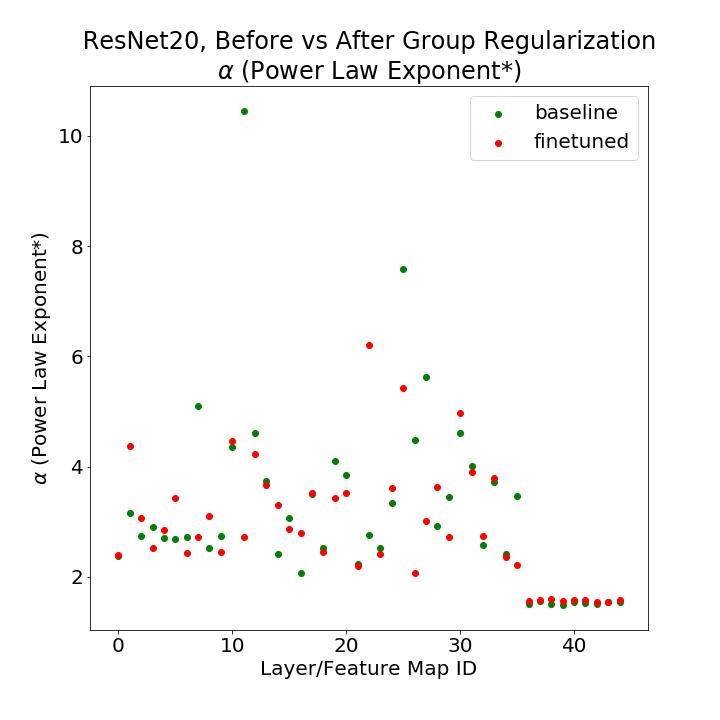
\includegraphics[width=4.0cm]{img/resnet4d_alphas.png}
      %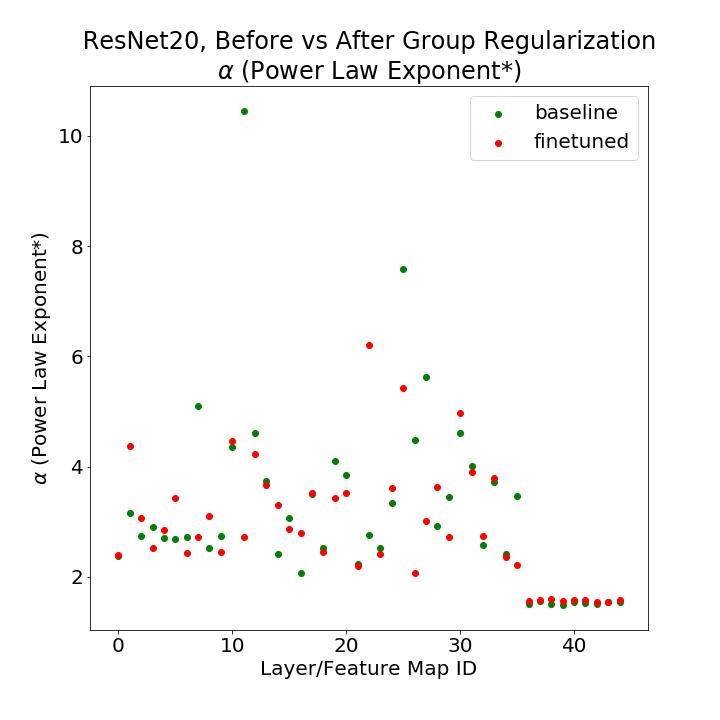
\includegraphics[width=4.5cm]{img/resnet4d_alphas.png}
      \label{fig:resnet204Dalpha}
   }
   \caption{%Correlation Flow.
            ResNet20, distilled with Group Regularization, as implemented in the \texttt{distiller} (4D\_regularized\_5Lremoved) pretrained models.  
            Log Spectral Norm ($\log\lambda_{max}$) and PL exponent ($\alpha$) for individual layers, versus layer id, for both baseline (before distillation, green) and fine-tuned (after distillation, red) pretrained models. 
           }
   \label{fig:resnet204D5L}
\end{figure}


%% %\paragraph{Layer Analysis: Behavior on Less Thoroughy Studied CV Models.}
%% \paragraph{Correlation Flow: PL vs. Norm Metrics.}
\paragraph{Scale Collapse; or How Distillation May Break Models.}

The similarity between norm-based metrics and PL-based metrics suggests a question: is the Weighted Alpha metric just a variation of the more familiar norm-based metrics?  %%, or does it capture something different?  
More generally, do fitted $\alpha$ values contain information not captured by norms? 
In examining hundreds of pretrained models, we have found several anamolies that demonsrate the power of our approach.
In particular, to show that $\alpha$ does capture something different, consider the following example, which looks at a compressed/distilled DNN model~\cite{CWZZ17_TR}.
In this example, we show that some distillation methods may actually \emph{break} models unexpectedly by introducing what we call \emph{Scale Collapse}, where several distilled layers have unexpectedly small Spectral Norms.

We consider ResNet20, trained on CIFAR10, before and after applying the Group Regularization distillation technique, as implemented in the \texttt{distiller} package~\cite{distiller}.
We analyze the pretrained 4D\_regularized\_5Lremoved baseline and fine-tuned models. 
The reported baseline test accuracies (Top1$=91.45$ and Top5$=99.75$) are better than the reported fine-tuned test accuracies (Top1$=91.02$ and Top5$=99.67$).  Because the baseline accuracy is greater,  the previous results on ResNet (Table~\ref{table:cv-models} and Figure~\ref{fig:cv2-accuracy}) suggests that the baseline Spectral Norms should be \emph{smaller} on average than the fine-tuned ones. \emph{The oppopsite is observed.}
%\michael{Do we have something backwards here: where we observed that the average norm to increase with decreasing test error (as it ``should'' not), whereas the average PL exponent $\alpha$ decreases (as ``expected'' from HT-SR Theory).  }
%In both cases (Frobenius norm results not shown), we observe the opposite.
\charles{WHy is this confusing? Call me...}
Figure~\ref{fig:resnet204D5L} presents the Spectral Norm (here denoted $\log\lambda_{max}$) and PL exponent ($\alpha$) for each individual layer weight matrix $\mathbf{W}$.%
\footnote{Here, we only include layer matrices or feature maps with $M\ge50$.}
On the other hand, the $\alpha$ values (in Figure~\ref{fig:resnet204Dalpha}) do not differ systematically between the baseline and fine-tuned models.
%\michael{Some comment about big jump in norm; but fix previous backwards question first.}--SEE BELOW
Also (not shown), the average (unweighted) baseline $\alpha$ is \emph{smaller} than the fine-tuned average (as predicted by HT-SR Theory, the basis of $\hat{\alpha}$).

(That being said, Figure~\ref{fig:resnet204Dalpha} also depcits two very large $\alpha\gg 6$ values for the baseline, but not for the fine-tuned, model.
This suggests the baseline model has at least two over-parameterized/under-trained layers, and that the distillation method does, in fact, improve the fine-tuned model by compressing these layers.)

The pretrained models in the \texttt{distiller} package have passed some quality metric, but they are much less well trodden than any of the 
VGG, ResNet, or DenseNet series.  %% we considered above.
While norms make good regularizers for a single model, there is no reason \emph{a priori} to expect them correlate so well with test accuracies across different models.
We do expect, however, the PL $\alpha$ to do so because it effectively measures the amount of correlation in the model~\cite{MM18_TR, MM19_HTSR_ICML, MM20_SDM}.
The reason for the anomalous behavior shown in 
Figure~\ref{fig:resnet204D5L}
is that the \texttt{distiller} Group Regularization technique 
%%has the unusual effect of increasing
spuriously increases the norms of the $\mathbf{W}$ pre-activation maps for at least two of the Conv2D layers.
This is difficult to diagnose by analyzing training/test curves, but it is easy to diagnose with our approach.


